\documentclass[acmsmall,screen,nonacm]{acmart}

\citestyle{acmauthoryear}

\usepackage{tabularx}
\usepackage{enumitem}
\usepackage{multirow}
\usepackage{tikz}
\usetikzlibrary{arrows.meta,positioning}

% Colours of the TikZ figures
\definecolor{edgec}{rgb}{0.3851,0.41255,0.44}
\definecolor{slate100}{rgb}{0.9451,0.96078,0.97647}
\definecolor{red100}{rgb}{0.99608,0.88628,0.88628}
\definecolor{teal100}{rgb}{0.8,0.98431,0.9451}
\definecolor{blue100}{rgb}{0.85883,0.91765,0.99608}
\definecolor{amber100}{rgb}{0.99608,0.95294,0.7804}
\definecolor{violet100}{rgb}{0.92941,0.91374,0.99608}
\definecolor{hdrc}{rgb}{0.12158,0.16078,0.2}
\definecolor{conc}{rgb}{0.47295,0.49648,0.52}
\definecolor{famO}{rgb}{0.7255,0.1098,0.1098}
\definecolor{famE}{rgb}{0.14511,0.38824,0.92157}
\definecolor{famT}{rgb}{0.85098,0.46667,0.02353}
\definecolor{famC}{rgb}{0.05882,0.46275,0.43137}
\definecolor{violetc}{rgb}{0.48627,0.22745,0.92941}
\definecolor{grayc}{rgb}{0.60393,0.64706,0.69412}
\definecolor{gray600}{rgb}{0.29727,0.32863,0.36}

\newcommand{\eff}{\mathrm{eff}}

\begin{document}

\title{Collectively Big, Locally Small}
\subtitle{Formalizing Small Data in Healthcare and Learning Privately Across Siloed Hospitals}

\author{Sancho Amaral Sim\~{o}es}
\authornote{Corresponding author.}
\email{sanchosimoes@student.dei.uc.pt}
\affiliation{%
  \institution{CISUC, DEI, FCTUC, University of Coimbra}
  \city{Coimbra}
  \country{Portugal}}

\author{Jo\~{a}o P. Vilela}
\email{jvilela@fc.up.pt}
\affiliation{%
  \institution{CISUC, DEI, FCTUC, University of Coimbra}
  \city{Coimbra}
  \country{Portugal}}
\affiliation{%
  \institution{CRACS/INESC TEC, DCS, FCUP, University of Porto}
  \city{Porto}
  \country{Portugal}}

\author{Pedro Henriques Abreu}
\email{pha@dei.uc.pt}
\affiliation{%
  \institution{CISUC, DEI, FCTUC, University of Coimbra}
  \city{Coimbra}
  \country{Portugal}}

\begin{abstract}
Health systems produce data at an enormous rate, yet most clinical learning problems are small. A rare disease registry holds a few hundred patients, an intensive care unit sees a handful of the outcome it wants to predict, a regional hospital owns a fraction of the cases needed to validate a model, and the data that would close the gap sit in other institutions that cannot legally or practically share them. ``Small data'' is invoked constantly in the literature but is rarely defined in a way that can be measured, compared, or reasoned about. This survey and position paper does four things. First, it gives a task-relative formal definition of small data through an effective sample size and a smallness index that combine learning-theoretic sample complexity with the clinical sample-size criteria used in prediction modeling. Second, it introduces a new two-axis taxonomy. The first axis classifies ten forms of scarcity in healthcare by the term of the smallness index they degrade, grouped into ontic, epistemic, temporal-contextual and custodial scarcity. The second axis classifies every remedy by the provenance of the information it injects (pooling, proxy, prior, unlabeled data, procurement, re-expression), and we prove that re-expression, which includes augmentation and synthetic data, cannot add information about the target that was not already present in the data or in the generator. Third, we code a curated corpus of 290 works on both axes and use it to review the solution families across imaging, electronic health records, omics and tabular data, to summarize the quantitative evidence, and to locate where it is thin. Only 18 of the 290 works are multi-institution studies, all of them on pooling, and temporal obsolescence, measurement poverty and stratum sparsity are barely addressed by any channel. Fourth, for sparse networks of hospitals that operate as data silos, we derive a privacy-preserving hierarchical borrowing scheme that runs by gossip over the existing collaboration graph without a central server. We show that it adds the same number of ``virtual patients'', $\sigma^2/(\tau^2+M)$, to every site, so that the smallest hospitals gain the most, that differential privacy enters only through the population-level estimate, and that the gossip phase incurs no additional privacy cost. We close with a research agenda.
\end{abstract}

\begin{CCSXML}
<ccs2012>
   <concept>
       <concept_id>10010147.10010257</concept_id>
       <concept_desc>Computing methodologies~Machine learning</concept_desc>
       <concept_significance>500</concept_significance>
       </concept>
   <concept>
       <concept_id>10010405.10010444.10010449</concept_id>
       <concept_desc>Applied computing~Health informatics</concept_desc>
       <concept_significance>500</concept_significance>
       </concept>
   <concept>
       <concept_id>10002978.10003029.10011150</concept_id>
       <concept_desc>Security and privacy~Privacy protections</concept_desc>
       <concept_significance>300</concept_significance>
       </concept>
 </ccs2012>
\end{CCSXML}

\ccsdesc[500]{Computing methodologies~Machine learning}
\ccsdesc[500]{Applied computing~Health informatics}
\ccsdesc[300]{Security and privacy~Privacy protections}

\keywords{small data, healthcare, effective sample size, taxonomy, federated learning, decentralized learning, differential privacy, hierarchical Bayes, data silos, rare diseases, foundation models, synthetic data}

\maketitle
\renewcommand{\shortauthors}{Sim\~{o}es et al.}

%% ===================================================================
\section{Introduction}\label{sec:intro}

The standard story of machine learning in medicine is a story about scale. Large labeled collections of retinal photographs, skin lesions and chest radiographs produced models that matched specialists on narrow tasks \cite{rajpurkar2022ai,topol2019high}, and the broader field learned that performance tends to grow predictably with data \cite{halevy2009unreasonable,hestness2017deep,kaplan2020scaling,sun2017revisiting}. The story is accurate for the problems it describes. It is not representative of the problems most clinicians and health systems actually face.

Consider what a typical clinical question looks like from the inside. Rare diseases are individually rare but collectively common: the Orphanet database lists more than six thousand of them, affecting an estimated 3.5\% to 5.9\% of the population \cite{nguengangwakap2020estimating}, and most have cohorts of tens or hundreds of patients worldwide \cite{banerjee2023machine,schaefer2020use}. Prediction models in common conditions are routinely built on a few dozen outcome events, which is why the clinical literature has spent three decades arguing over events per variable \cite{peduzzi1996simulation,riley2019minimumsample,smeden2019sample}. During the first months of COVID-19, hundreds of models were developed from small, local, convenience samples, and systematic reviews found nearly all of them to be at high risk of bias and none fit for clinical use \cite{roberts2021common,wynants2020prediction}. Even large systems turn small at the point of deployment: a proprietary sepsis model used in hundreds of hospitals achieved an area under the curve of 0.63 on external validation and missed two thirds of sepsis cases \cite{wong2021external}, and convolutional networks for pneumonia learned to recognize the hospital that produced an image rather than the disease \cite{zech2018variable}.

These failures share a structure. Health data are abundant in aggregate and scarce where they are needed: for the specific outcome, in the specific subgroup, at the specific site, in the current period, with labels. They are also fragmented. Every hospital holds a slice of the population under its own legal, ethical and technical constraints \cite{cohen2018hipaa,gdpr2016,price2019privacy}, and the European Health Data Space regulation \cite{ehds2025} is a recent recognition that this fragmentation is itself a policy problem. The consequence is a paradox that motivates this paper: \emph{healthcare is collectively big and locally small}.

The term ``small data'' appears in social science \cite{kitchin2015small}, in personal health \cite{estrin2014small,hekler2019we}, in statistics \cite{faraway2018when}, and in hundreds of applied papers. It is almost always used informally, as a synonym for ``fewer samples than we would like''. Three consequences follow. Methods are compared across problems whose difficulty is not comparable. Remedies that cannot work in a given setting are applied anyway, as when synthetic data is expected to compensate for a cohort that does not contain the relevant information. And the specific case of many small, isolated institutions, which is the default organizational form of healthcare, is treated either as a federated learning problem with a central server that often does not exist, or not at all.

\paragraph{Contributions} This paper is both a survey and a position paper. Its contributions are as follows.
\begin{enumerate}[leftmargin=*,itemsep=2pt]
\item \textbf{A formal definition.} We define small data relative to a task, through an \emph{effective sample size} $n^{\eff}$ that accounts for clustering, missing labels, label noise, distribution shift and outcome rarity, and a \emph{smallness index} $\sigma = n^{\star}/n^{\eff}$ that compares it with the sample complexity $n^{\star}$ of the task (Section~\ref{sec:definition}). The definition assembles known ingredients (Kish's design effect, the sample complexity of learning with label noise, and the sample-size criteria used for clinical prediction models) into one task-relative quantity. It is a first-order heuristic for diagnosis and comparison, not a new estimator.
\item \textbf{A new taxonomy.} We propose the Scarcity-Provenance taxonomy (Sections~\ref{sec:scarcity} and~\ref{sec:provenance}). Its first axis classifies ten forms of scarcity in healthcare by the term of $\sigma$ they degrade. Its second axis classifies remedies by where the missing information comes from. We prove a ``no free lunch'' result for re-expression (Proposition~\ref{prop:nfl}) that explains formally why augmentation and synthetic data cannot by themselves solve a small-data problem.
\item \textbf{A coded survey.} We classify a curated corpus of 290 works on both axes (Section~\ref{sec:method}, Appendix~\ref{app:corpus}), review the solutions channel by channel (Section~\ref{sec:solutions}), and compare where the literature has actually worked with where the taxonomy says it could, which exposes specific empty cells (Section~\ref{sec:evidence}).
\item \textbf{A blueprint for siloed hospital networks.} For sparse networks of hospitals without a trusted central server, we derive a privacy-preserving hierarchical borrowing scheme with closed-form risk, explicit privacy cost and convergence on sparse graphs (Section~\ref{sec:blueprint}), and argue that it is a principled default for this setting. The ingredients are standard; their combination for serverless hospital networks, and its empirical evaluation, are what remain open.
\item \textbf{A research agenda} with concrete open problems (Section~\ref{sec:agenda}).
\end{enumerate}

\begin{figure*}[t]
\centering
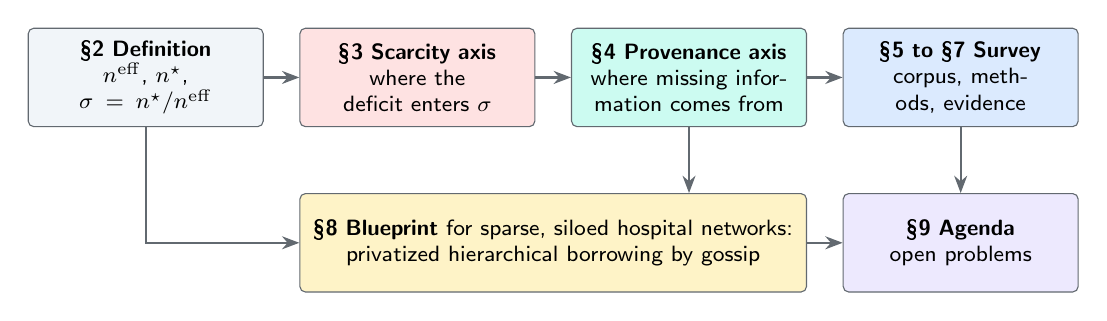
\begin{tikzpicture}[x=1bp,y=1bp,
  box/.style={fill=#1,draw=edgec,line width=0.4pt,rounded corners=2pt},
  btxt/.style={align=center,font=\footnotesize\sffamily,inner sep=0pt,text width=2.7cm},
  arr/.style={draw=edgec,line width=0.8pt,-{Stealth[length=2.2mm]}}]
\path[box=slate100] (-42.297,-17.717) rectangle (42.297,17.717);
\path[box=red100] (55.499,-17.717) rectangle (140.094,17.717);
\path[box=teal100] (153.295,-17.717) rectangle (237.890,17.717);
\path[box=blue100] (251.092,-17.717) rectangle (335.687,17.717);
\path[box=amber100] (55.499,-77.245) rectangle (237.890,-41.812);
\path[box=violet100] (251.092,-77.245) rectangle (335.687,-41.812);
\node[btxt] at (0,0) {\textbf{\S2 Definition}\\ $n^{\eff}$, $n^{\star}$, $\sigma = n^{\star}/n^{\eff}$};
\node[btxt] at (97.797,0) {\textbf{\S3 Scarcity axis}\\ where the deficit enters $\sigma$};
\node[btxt] at (195.594,0) {\textbf{\S4 Provenance axis}\\ where missing information comes from};
\node[btxt] at (293.390,0) {\textbf{\S5 to \S7 Survey}\\ corpus, methods, evidence};
\node[btxt,text width=6.2cm] at (146.695,-59.528) {\textbf{\S8 Blueprint} for sparse, siloed hospital networks: privatized hierarchical borrowing by gossip};
\node[btxt] at (293.390,-59.528) {\textbf{\S9 Agenda}\\ open problems};
\draw[arr] (42.497,0) -- (55.299,0);
\draw[arr] (140.294,0) -- (153.095,0);
\draw[arr] (238.090,0) -- (250.892,0);
\draw[arr] (195.593,-17.916) -- (195.593,-41.612);
\draw[arr] (293.390,-17.916) -- (293.390,-41.612);
\draw[arr] (238.090,-59.528) -- (250.892,-59.528);
\draw[arr] (0,-17.916) -- (0,-59.528) -- (55.299,-59.528);
\end{tikzpicture}
\caption{Structure of the paper. The definition of Section~\ref{sec:definition} produces the two axes of the taxonomy, which serve as the coding scheme of the survey and shape the design of the blueprint.}
\label{fig:structure}
\end{figure*}

\paragraph{Scope and method} We cover supervised and semi-supervised prediction from clinical data: imaging, structured electronic health records (EHR), clinical text, omics and tabular registries. We do not cover causal effect estimation from small trials in depth, although several of our results apply to it. How the corpus was assembled and coded, and what remains to be done before the review can be called systematic, is described in Section~\ref{sec:method}. Existing surveys cover individual families, such as federated learning in healthcare \cite{nguyen2022federated,rieke2020future,xu2021federated}, few-shot learning \cite{wang2020generalizing}, meta-learning \cite{hospedales2022meta}, imperfect medical datasets \cite{cheplygina2019not,tajbakhsh2020embracing}, informed machine learning \cite{rueden2023informed} and synthetic data \cite{chen2021synthetic,jordon2022synthetic}. Among the surveys we found, none defines small data formally, none organizes remedies by information provenance, and none treats the sparse, serverless hospital network as a first-class setting.

\paragraph{How the parts connect} The paper is built as a single argument, shown in Figure~\ref{fig:structure}. We first make smallness measurable (Section~\ref{sec:definition}). The terms of that measure tell us \emph{why} a dataset is small, which gives the scarcity axis of the taxonomy (Section~\ref{sec:scarcity}). Knowing why points to \emph{where} the missing information could come from, which gives the provenance axis (Section~\ref{sec:provenance}). The two axes then serve as the coding scheme for a corpus of 290 works (Section~\ref{sec:method}), which organizes the survey of existing methods (Section~\ref{sec:solutions}) and the reading of their evidence (Section~\ref{sec:evidence}). The gaps that this reading exposes, together with the definition of siloed smallness from Section~\ref{sec:definition}, determine the design of the blueprint (Section~\ref{sec:blueprint}), and what remains unsolved becomes the agenda (Section~\ref{sec:agenda}).

%% ===================================================================
\section{What Is Small Data? A Formal Account}\label{sec:definition}

The paradox of the introduction can only be studied once it can be measured. This section turns ``small'' from an adjective into a quantity, and that quantity is the thread that runs through the rest of the paper.

\begin{table}[t]
\caption{Main notation.}
\label{tab:notation}
\small
\begin{tabularx}{\linewidth}{@{}lX@{}}
\toprule
Symbol & Meaning\\
\midrule
$\mathcal{T}=(P,\mathcal{H},\ell,\varepsilon,\delta)$ & learning task: target distribution, hypothesis class, loss, tolerance, confidence\\
$n$, $n^{\eff}$ & nominal number of records; effective sample size (Definition~\ref{def:ess})\\
$n^{\star}_{\mathcal{T}}$ & sample complexity of $\mathcal{T}$ (Definition~\ref{def:samplecomplexity})\\
$\sigma_{\mathcal{T}}(\mathcal{D})$ & smallness index $n^{\star}_{\mathcal{T}}/n^{\eff}(\mathcal{D})$ (Definition~\ref{def:smallness})\\
DEFF, $\rho_L$, $\eta$, $\rho_S$, $\pi$ & design effect, labeled fraction, label noise rate, shift efficiency, outcome prevalence\\
$K$, $\mathcal{G}=(V,E)$, $W$ & number of hospitals, collaboration graph, gossip matrix\\
$\theta_k$, $\hat{\theta}_k$, $v_k=\sigma^2/n_k$ & parameter of site $k$, its local estimate, and the variance of that estimate\\
$\mu$, $\tau^2$, $M$ & population mean of site parameters, between-site heterogeneity, mean squared error of the estimate of $\mu$\\
$(\epsilon,\delta)$ & differential privacy parameters (written $\epsilon$ to distinguish them from the tolerance $\varepsilon$)\\
\bottomrule
\end{tabularx}
\end{table}

\subsection{Existing notions}

Informal notions of small data fall into three groups. The first is \emph{absolute}: a dataset is small if it has few records, often with arbitrary cut-offs such as a few hundred or a few thousand. This ignores the task. One thousand patients is a lot for estimating a mean blood pressure and very little for a 50-predictor model of a 2\% outcome. The second is \emph{relational}, as in Kitchin and Lauriault's contrast between small data, collected for a specific question with controlled sampling, and big data, which is exhaustive, fine-grained and collected as a by-product \cite{kitchin2015small}. Estrin's ``n of 1'' \cite{estrin2014small} and the small data paradigm of \citet{hekler2019we} belong here, stressing individual-level inference rather than population scale. \citet{faraway2018when} show that a small designed sample can beat a large biased one, which is a statement about information, not about size. The third group is \emph{criterion-based} and comes from clinical prediction research: a dataset is adequate if it contains at least ten events per candidate predictor \cite{peduzzi1996simulation}, or more defensibly if it meets the criteria of \citet{riley2019minimumsample}, which bound overfitting, optimism in apparent fit and imprecision of the intercept \cite{riley2020calculating,smeden2019sample}.

Only the third group is quantitative, and it is tied to regression models. Learning theory provides the general quantity, sample complexity, but it ignores the specific ways in which clinical data lose information. We combine the two.

\subsection{Setup and notation}

A learning \emph{task} is a tuple $\mathcal{T}=(P,\mathcal{H},\ell,\varepsilon,\delta)$, where $P$ is a distribution over $\mathcal{X}\times\mathcal{Y}$ describing the target population at the point of use, $\mathcal{H}$ a hypothesis class, $\ell$ a loss bounded in $[0,1]$, and $(\varepsilon,\delta)$ the required excess risk and confidence. The risk of $h$ is $R(h)=\mathbb{E}_{(x,y)\sim P}\,\ell(h(x),y)$. Notation used throughout is collected in Table~\ref{tab:notation}.

\begin{definition}[Sample complexity of a task]\label{def:samplecomplexity}
The sample complexity $n^{\star}_{\mathcal{T}}$ is the smallest $n$ for which there is a learner $A$ such that, for $\mathcal{D}\sim P^n$ independent and identically distributed (i.i.d.) and fully and correctly labeled,
\[
\Pr_{\mathcal{D}\sim P^n}\left[R(A(\mathcal{D})) - \inf_{h\in\mathcal{H}} R(h) \le \varepsilon\right] \;\ge\; 1-\delta.
\]
\end{definition}

$n^{\star}$ is rarely known exactly, but it has usable proxies. For agnostic learning of a class with VC dimension $d$, $n^{\star}=\Theta\bigl((d+\log(1/\delta))/\varepsilon^2\bigr)$ \cite{shalevshwartz2014understanding}, and data-dependent versions replace $d$ with Rademacher complexity \cite{bartlett2002rademacher}. For logistic and survival prediction models, the criteria of Riley et al. give closed forms. Their first criterion, which targets a global shrinkage factor $S$ (typically $0.9$) for a model with $p$ candidate parameters and anticipated Cox-Snell $R^2_{\mathrm{CS}}$, is
\begin{equation}\label{eq:riley}
n^{\star} \;\ge\; \frac{p}{(S-1)\,\ln\bigl(1-R^2_{\mathrm{CS}}/S\bigr)} \qquad \text{\cite{riley2019minimumsample}.}
\end{equation}
Either way, $n^{\star}$ grows with model complexity and with the precision demanded, and for binary outcomes it is driven by the number of events rather than the number of patients.

\subsection{Effective sample size}

Clinical records are not i.i.d., not all labeled, not all correctly labeled, and not drawn from the population where the model will be used. Each of these reduces the information a record carries.

\begin{definition}[Effective sample size]\label{def:ess}
Let $\mathcal{D}$ contain $n$ records. Its effective sample size $n^{\eff}(\mathcal{D})$ is the number of i.i.d., correctly labeled records drawn from the target distribution $P$ that would give an estimator with the same variance as the one obtained from $\mathcal{D}$. To first order, when the mechanisms below act independently,
\begin{equation}\label{eq:neff}
n^{\eff} \;=\; n\cdot\underbrace{\frac{1}{\mathrm{DEFF}}}_{\text{clustering}}\cdot\underbrace{\rho_L}_{\text{labels}}\cdot\underbrace{(1-2\eta)^2}_{\text{label noise}}\cdot\underbrace{\rho_S}_{\text{shift}},
\end{equation}
where $\mathrm{DEFF}=1+(\bar{m}-1)\,\mathrm{ICC}$ is the design effect for $\bar{m}$ records per patient with intra-class correlation ICC \cite{kish1965survey}; $\rho_L$ is the fraction of records with labels missing completely at random; $\eta<1/2$ is a symmetric label-noise rate, whose effect on sample complexity scales as $(1-2\eta)^{-2}$ \cite{angluin1988learning}; and $\rho_S=(\sum_i w_i)^2/(n\sum_i w_i^2)$ is Kish's efficiency of the importance weights $w_i=p_P(x_i)/p_{\mathcal{D}}(x_i)$ needed to transport the sample to $P$ \cite{kish1965survey}. For a binary outcome with prevalence $\pi$, the information about the decision boundary is controlled by the minority class, $n^{\eff}_{\mathrm{ev}}=n^{\eff}\cdot\min(\pi,1-\pi)$.
\end{definition}

Equation~\eqref{eq:neff} is deliberately simple. Each factor is a standard, estimable quantity, and each can be replaced by a more refined estimator (for instance, the fraction of missing information under multiple imputation) without changing the structure. The factors multiply because each is a ratio of variances under an independent mechanism; when mechanisms interact, the product is an approximation. None of the factors is new, and Equation~\eqref{eq:neff} should be read as a first-order heuristic: it is meant to compare datasets and to show where information is lost, not to replace a variance computed for a specific estimator. What it adds is a single place where the clinical and the learning-theoretic notions of sample size meet, relative to a task.

\begin{definition}[Smallness index]\label{def:smallness}
The smallness index of a dataset $\mathcal{D}$ for task $\mathcal{T}$ is $\sigma_{\mathcal{T}}(\mathcal{D})=n^{\star}_{\mathcal{T}}/n^{\eff}(\mathcal{D})$. The dataset is \emph{small for} $\mathcal{T}$ when $\sigma_{\mathcal{T}}(\mathcal{D})>1$. We call the regimes $\sigma\le 1$ \emph{sufficient}, $1<\sigma\le 10$ \emph{strained}, $10<\sigma\le 100$ \emph{small}, and $\sigma>100$ \emph{extreme}.
\end{definition}

The thresholds are conventions, chosen so that each regime corresponds to a qualitatively different strategy. In the strained regime, regularization, simpler models and careful validation usually close the gap. In the small regime, information has to be imported from outside the dataset. In the extreme regime, only strong priors or pooling at a scale beyond any single institution will help.

\begin{example}[An ICU deterioration model]\label{ex:icu}
A hospital has $n=2{,}000$ ICU stays from patients with on average $\bar{m}=1.6$ stays each and $\mathrm{ICC}=0.5$, so $\mathrm{DEFF}=1.3$. Seventy percent of stays have an adjudicated outcome, adjudication disagrees with a reference standard in 10\% of cases, and the case mix differs from the deployment population with Kish efficiency $0.6$. By Equation~\eqref{eq:neff}, $n^{\eff}\approx 414$, and at an outcome prevalence of 8\% the dataset contains about 33 effective events. For a model with $p=20$ parameters and an anticipated $R^2_{\mathrm{CS}}$ of 15\% of its maximum, Equation~\eqref{eq:riley} gives $n^{\star}\approx 2{,}707$. Hence $\sigma\approx 6.5$: a dataset that looks moderate is strained, close to small. Figure~\ref{fig:deflation} shows the decomposition.
\end{example}

\begin{figure}[t]
\centering
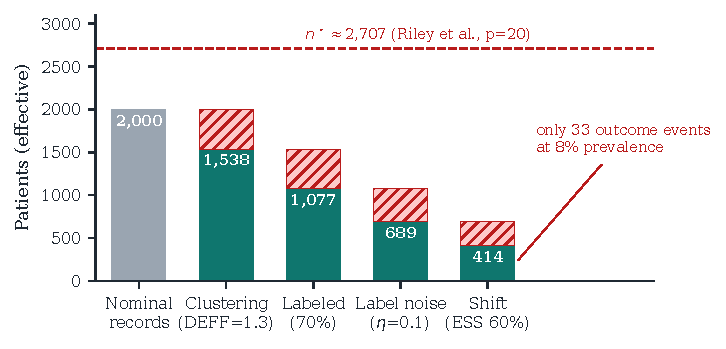
\includegraphics[width=0.8\linewidth]{figures/fig_deflation}
\caption{Deflation of a nominal sample of 2,000 ICU stays into an effective sample size (Example~\ref{ex:icu}). Hatched segments show the information lost to each mechanism of Equation~\eqref{eq:neff}. The dashed line is the sample size required by the first criterion of \citet{riley2019minimumsample} for a 20-parameter model at 8\% prevalence.}
\label{fig:deflation}
\end{figure}

\subsection{Siloed smallness}

The definitions so far concern one dataset. Healthcare adds a second level: data that would be sufficient together are held separately.

\begin{definition}[Siloed smallness]\label{def:siloed}
Let $\mathcal{D}_1,\dots,\mathcal{D}_K$ be held by $K$ custodians and let $\mathcal{D}_{\cup}$ be their union. The task $\mathcal{T}$ is \emph{siloed-small} if $\sigma_{\mathcal{T}}(\mathcal{D}_k)>1$ for every $k$ while $\sigma_{\mathcal{T}}(\mathcal{D}_{\cup})\le 1$, where $n^{\eff}(\mathcal{D}_{\cup})$ is computed after accounting for the heterogeneity across custodians (the shift factor $\rho_S$ of Equation~\eqref{eq:neff} applied to the mixture). The ratio $\Gamma=\min_k \sigma_{\mathcal{T}}(\mathcal{D}_k)/\sigma_{\mathcal{T}}(\mathcal{D}_{\cup})$ is the \emph{custodial gap}.
\end{definition}

A siloed-small task can be solved in principle without collecting a single new patient; the obstacle is access. A task that is small even for $\mathcal{D}_{\cup}$ is \emph{intrinsically small}, and no amount of collaboration among the existing custodians will solve it. Rare disease work often sits between the two. The distinction matters because the remedies are different, and because heterogeneity between custodians can make $n^{\eff}(\mathcal{D}_{\cup})$ much smaller than $\sum_k n^{\eff}(\mathcal{D}_k)$. Section~\ref{sec:blueprint} makes this precise.

\subsection{Why healthcare is a special case}

Small data exist in every field, but five properties make healthcare unusual. \emph{Stakes are asymmetric}: errors fall on patients, so the tolerance $\varepsilon$ is small and the required $n^{\star}$ is large. \emph{Labels are expensive and delayed}: ground truth often needs specialist review, biopsy, or months of follow-up \cite{willemink2020preparing}. \emph{Heterogeneity is structural}: devices, coding practices, referral patterns and populations differ across sites in ways that models detect and exploit \cite{finlayson2021clinician,gichoya2022ai,zech2018variable}. \emph{Re-identification risk is high}: Rocher et al. estimate that 99.98\% of Americans would be correctly re-identified in any dataset using 15 demographic attributes \cite{rocher2019estimating}, which undermines de-identification as a basis for sharing \cite{price2019privacy,sweeney2002k}. And \emph{subgroups matter}: performance in a minority subgroup is a clinical and ethical requirement, not a secondary metric \cite{chen2021ethical,obermeyer2019dissecting}. Each subgroup has its own, smaller $n^{\eff}$.

\begin{figure*}[t]
\centering
\resizebox{\linewidth}{!}{%
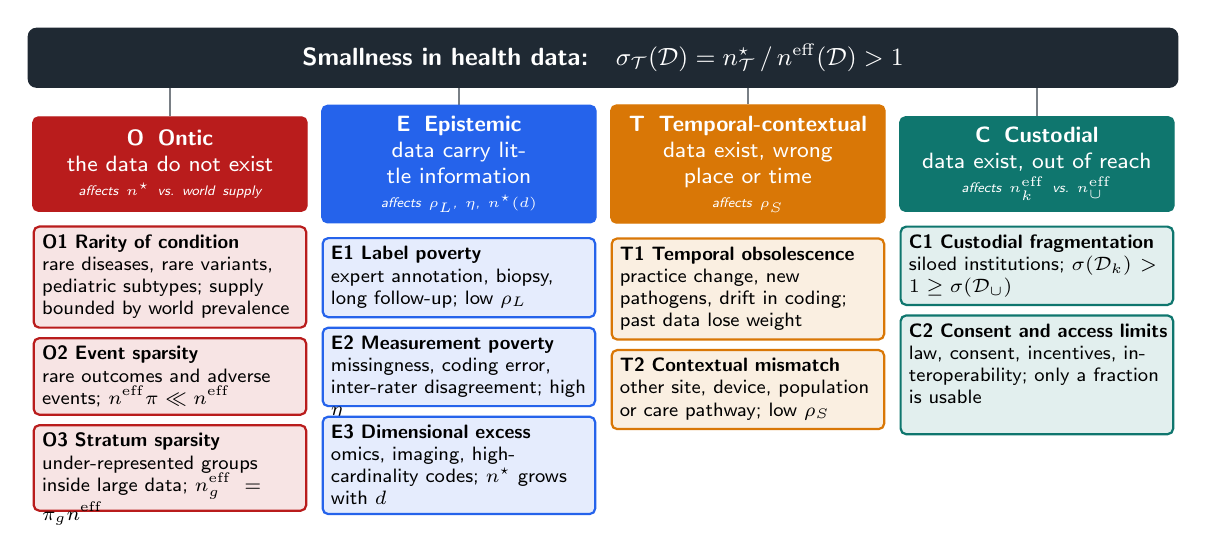
\begin{tikzpicture}[x=1bp,y=1bp,
  hdr/.style={fill=hdrc,draw=hdrc,line width=0.4pt,rounded corners=3pt},
  fam/.style={fill=#1,draw=#1,line width=0.4pt,rounded corners=2pt},
  cls/.style={fill=#1!12,draw=#1,line width=0.8pt,rounded corners=2pt},
  famtxt/.style={text=white,align=center,font=\footnotesize\sffamily,inner sep=0pt,text width=88pt},
  clstxt/.style={text width=93.75pt,align=left,font=\scriptsize\sffamily,inner sep=0pt,anchor=north west},
  con/.style={draw=conc,line width=0.8pt}]
\path[hdr] (-206.932,-10.630) rectangle (206.932,10.630);
\node[text=white,font=\small\sffamily\bfseries,inner sep=0pt] at (0,0)
  {Smallness in health data:\quad $\sigma_{\mathcal{T}}(\mathcal{D}) = n^{\star}_{\mathcal{T}}\,/\,n^{\eff}(\mathcal{D}) > 1$};
\foreach \x/\y in {-155.907/-21.061,-51.875/-16.908,52.158/-16.783,156.191/-21.046}
  \draw[con] (\x,-10.829) -- (\x,\y);
\path[fam=famO] (-205.292,-55.276) rectangle (-106.523,-21.260);
\path[fam=famE] (-101.259,-59.429) rectangle (-2.491,-17.108);
\path[fam=famT] (2.774,-59.555) rectangle (101.542,-16.982);
\path[fam=famC] (106.807,-55.292) rectangle (205.575,-21.245);
\node[famtxt] at (-155.907,-38.268) {\textbf{O}\hspace{4.88pt}\textbf{Ontic}\\ the data do not exist\\[-1pt] {\tiny\itshape affects $n^{\star}$ vs.\ world supply}};
\node[famtxt] at (-51.875,-38.268) {\textbf{E}\hspace{4.88pt}\textbf{Epistemic}\\ data carry little information\\[-1pt] {\tiny\itshape affects $\rho_L$, $\eta$, $n^{\star}(d)$}};
\node[famtxt] at (52.158,-38.268) {\textbf{T}\hspace{4.88pt}\textbf{Temporal-contextual}\\ data exist, wrong place or time\\[-1pt] {\tiny\itshape affects $\rho_S$}};
\node[famtxt] at (156.191,-38.268) {\textbf{C}\hspace{4.88pt}\textbf{Custodial}\\ data exist, out of reach\\[-1pt] {\tiny\itshape affects $n^{\eff}_k$ vs.\ $n^{\eff}_{\cup}$}};
\newcommand\cls[6]{\path[cls=#1] (#2,#3) rectangle (#4,#5);
  \node[clstxt] at ({#2+2.79},{#5-2.79}) {#6};}
\cls{famO}{-204.960}{-97.155}{-106.855}{-60.777}{\textbf{O1 Rarity of condition}\\ rare diseases, rare variants, pediatric subtypes; supply bounded by world prevalence}
\cls{famO}{-204.960}{-128.483}{-106.855}{-100.955}{\textbf{O2 Event sparsity}\\ rare outcomes and adverse events; $n^{\eff}\pi \ll n^{\eff}$}
\cls{famO}{-204.960}{-163.055}{-106.855}{-132.283}{\textbf{O3 Stratum sparsity}\\ under-represented groups inside large data; $n^{\eff}_g = \pi_g n^{\eff}$}
\cls{famE}{-100.927}{-93.383}{-2.822}{-64.930}{\textbf{E1 Label poverty}\\ expert annotation, biopsy, long follow-up; low $\rho_L$}
\cls{famE}{-100.927}{-125.416}{-2.822}{-97.183}{\textbf{E2 Measurement poverty}\\ missingness, coding error, inter-rater disagreement; high $\eta$}
\cls{famE}{-100.927}{-164.270}{-2.822}{-129.215}{\textbf{E3 Dimensional excess}\\ omics, imaging, high-cardinality codes; $n^{\star}$ grows with $d$}
\cls{famT}{3.106}{-101.433}{101.210}{-65.055}{\textbf{T1 Temporal obsolescence}\\ practice change, new pathogens, drift in coding; past data lose weight}
\cls{famT}{3.106}{-133.686}{101.210}{-105.233}{\textbf{T2 Contextual mismatch}\\ other site, device, population\\ or care pathway; low $\rho_S$}
\cls{famC}{107.138}{-88.976}{205.243}{-60.793}{\textbf{C1 Custodial fragmentation}\\ siloed institutions; $\sigma(\mathcal{D}_k) > 1 \geq \sigma(\mathcal{D}_{\cup})$}
\cls{famC}{107.138}{-135.520}{205.243}{-92.776}{\textbf{C2 Consent and access limits}\\ law, consent, incentives, interoperability; only a fraction is usable}
\end{tikzpicture}}
\caption{The scarcity axis of the Scarcity-Provenance taxonomy. Families are defined by the term of the smallness index they degrade; the ten classes are the forms these take in healthcare.}
\label{fig:scarcity}
\end{figure*}

\paragraph{From measurement to diagnosis} The smallness index tells us \emph{how} small a dataset is for a task. It does not yet tell us \emph{why}, and the why matters: a low $\rho_L$, a small $\pi$ and a large custodial gap all raise $\sigma$, but each calls for a different response. The next section uses the structure of $\sigma$ itself to classify the causes.

%% ===================================================================
\section{The Scarcity Axis: Where the Deficit Comes From}\label{sec:scarcity}

The first axis of our taxonomy answers the question \emph{why is this dataset small?} Existing classifications tend to mix causes (rare disease), symptoms (class imbalance) and remedies (few-shot learning). We instead classify scarcity by the term of the smallness index it degrades. This makes the classes operational, because each one points to a specific quantity that can be estimated. They are not mutually exclusive. Rarity of condition (O1) and event sparsity (O2) both lower the effective number of events, contextual mismatch (T2) and custodial fragmentation (C1) usually arrive together, and a single cohort can be label-poor and high-dimensional at once. A dataset therefore has a \emph{profile} over the ten classes, and that profile is more informative than any single label. This is also how we code the literature in Section~\ref{sec:method}: a work can target several classes.

\subsection{Ontic scarcity (O): the data do not exist}

Ontic scarcity is a property of the world, not of the dataset. More effort spent on collection or access will not remove it, only reduce it.

\textbf{O1, rarity of condition.} For a disease with worldwide prevalence $q$, the total supply of cases is bounded by $qN_{\mathrm{world}}$, and in practice by the fraction diagnosed and recorded. When $n^{\star}$ approaches that bound, the task is intrinsically small in the sense of Definition~\ref{def:siloed}. This is the situation of many of the conditions cataloged by Orphanet \cite{nguengangwakap2020estimating}, and the reason machine learning in rare diseases relies so heavily on transfer, knowledge and international pooling \cite{banerjee2023machine,schaefer2020use}.

\textbf{O2, event sparsity.} The condition may be common, but the outcome of interest is rare: in-hospital cardiac arrest, a severe adverse drug reaction, a post-operative complication. The number of patients is large but the effective number of events $n^{\eff}\pi$ is small, which is what drives the sample-size criteria \cite{peduzzi1996simulation,riley2019minimumsample}. Oversampling or reweighting changes the decision threshold, not the information.

\textbf{O3, stratum sparsity.} Within a large dataset, a subgroup $g$ with share $\pi_g$ has $n^{\eff}_g=\pi_g n^{\eff}$. Clinically meaningful subgroups (by ancestry, sex, age band, comorbidity or disease subtype) are often small even when the whole is not. Failures concentrated in such strata have been called hidden stratification \cite{oakdenrayner2020hidden}, and the related fairness failures are well documented \cite{chen2021ethical,obermeyer2019dissecting}.

\subsection{Epistemic scarcity (E): the data carry little information}

Here the patients exist and are recorded, but each record says less about the target than it could.

\textbf{E1, label poverty.} Unlabeled images, notes and signals are cheap, but labels need specialist time, invasive confirmation, or follow-up long enough for the outcome to occur \cite{willemink2020preparing}. Label poverty acts through $\rho_L$. It is the scarcity class for which semi-supervised, self-supervised and weakly supervised learning were developed \cite{cheplygina2019not,tajbakhsh2020embracing}.

\textbf{E2, measurement poverty.} Missing values that are not missing at random, billing codes that reflect reimbursement more than pathology, and disagreement between raters all reduce the information per record. In Equation~\eqref{eq:neff} this acts through $\eta$ and through the missing-information fraction.

\textbf{E3, dimensional excess.} Genomic, transcriptomic and imaging data have $d\gg n$. In this case $n^{\star}$ grows with $d$, often faster than any realistic cohort, unless strong structural assumptions such as sparsity are imposed \cite{buhlmann2011statistics,tibshirani1996regression}. Dimensional excess is the only class in which smallness can be created by the choice of representation, and therefore partly removed by changing it.

\subsection{Temporal-contextual scarcity (T): the data are about somewhere else}

\textbf{T1, temporal obsolescence.} Treatment guidelines, coding systems, assays and pathogens change. Data collected before a change are partly irrelevant afterwards, so the usable window is shorter than the archive. The early COVID-19 literature is an extreme case \cite{roberts2021common,wynants2020prediction}.

\textbf{T2, contextual mismatch.} A model trained at one site, scanner or population meets a different distribution at deployment \cite{finlayson2021clinician,koh2021wilds}. In Equation~\eqref{eq:neff} this is the factor $\rho_S$, which can be close to zero when supports barely overlap. Learning theory makes the same point through the divergence term in domain adaptation bounds \cite{bendavid2010theory}. External validation studies show the effect directly \cite{debray2015new,wong2021external,zech2018variable}.

\subsection{Custodial scarcity (C): the data are out of reach}

\textbf{C1, custodial fragmentation.} The information exists and is relevant, but is distributed across institutions that do not pool it. This is the silo problem formalized in Definition~\ref{def:siloed}, and the setting of Section~\ref{sec:blueprint}.

\textbf{C2, consent and access limits.} Even inside one institution, only part of the data can be used for a given purpose, because of consent scope, legal basis, governance review, or simply the absence of interoperable extraction \cite{cohen2018hipaa,gdpr2016,mandel2016smart}. Common data models such as OMOP and the OHDSI network \cite{hripcsak2015observational,overhage2012validation} and the FAIR principles \cite{wilkinson2016fair} attack the interoperability side of C2.

\begin{table}[t]
\caption{Scarcity classes, the quantity that measures each, and the characteristic failure when it is ignored.}
\label{tab:scarcity}
\small
\begin{tabularx}{\linewidth}{@{}lXX@{}}
\toprule
Class & What to estimate & Typical failure if ignored\\
\midrule
O1 Rarity of condition & world supply $qN_{\mathrm{world}}$ vs.\ $n^{\star}$ & optimistic results from a single centre that do not replicate\\
O2 Event sparsity & effective events $n^{\eff}\pi$ & overfitting, miscalibrated risks \cite{riley2019minimumsample}\\
O3 Stratum sparsity & $n^{\eff}_g$ for each relevant group $g$ & hidden stratification, subgroup harm \cite{oakdenrayner2020hidden}\\
E1 Label poverty & labeled fraction $\rho_L$, label delay & models trained only on the easy, labeled cases\\
E2 Measurement poverty & noise rate $\eta$, missingness mechanism & learning the documentation process, not the disease\\
E3 Dimensional excess & $d/n^{\eff}$, intrinsic dimension & spurious signatures, unstable feature selection\\
T1 Temporal obsolescence & time-sliced performance & silent decay after deployment\\
T2 Contextual mismatch & Kish efficiency $\rho_S$, site-held-out error & shortcut learning, external failure \cite{zech2018variable}\\
C1 Custodial fragmentation & custodial gap $\Gamma$ & many under-powered single-site models\\
C2 Consent and access limits & usable fraction per purpose & selection bias in the usable subset\\
\bottomrule
\end{tabularx}
\end{table}

\paragraph{Using the scarcity profile} Table~\ref{tab:scarcity} summarizes the ten classes with the quantity to estimate for each and the characteristic failure when it is ignored. We suggest that studies report this profile alongside $n^{\eff}$ and $\sigma$. It takes a few lines and would make results across small-data papers comparable for the first time.

\paragraph{From diagnosis to remedy} A scarcity profile identifies which factor of $\sigma$ is degraded, but not how to repair it. Every repair has to bring in information about the target from somewhere, and the possible sources are limited. The second axis of the taxonomy, introduced next, classifies remedies by that source.

%% ===================================================================
\section{The Provenance Axis: Where the Missing Information Comes From}\label{sec:provenance}

The second axis of the taxonomy classifies remedies, and it is the axis along which the rest of the paper is organized. Existing surveys group methods by technique (``generative models'', ``transfer learning'', ``federated learning''). Technique is the wrong primitive for small data, because two techniques that look different can draw on the same source of information, and two that look alike can draw on different ones. A GAN trained on the local cohort and a GAN pretrained on a million public images are both ``synthetic data'', but only the second brings anything new. We therefore classify remedies by the \emph{provenance} of the information they add.

\subsection{A conservation principle}

Let $\theta$ denote the unknown quantity we want to learn: a parameter, a regression function, or a decision rule for the target population. Let $\mathcal{D}$ be the local data and let $M$ denote any external resource used by a method, such as a pretrained network, a knowledge base, or a published risk score.

\begin{proposition}[No free lunch for re-expression]\label{prop:nfl}
Let $\tilde{\mathcal{D}}=g(\mathcal{D},M,U)$ be any dataset produced by a (possibly randomized) procedure $g$, where $U$ is randomness independent of $(\theta,\mathcal{D},M)$. Then
\[
I(\theta;\mathcal{D},\tilde{\mathcal{D}}) \;\le\; I(\theta;\mathcal{D},M).
\]
In particular, if $M$ is independent of $(\theta,\mathcal{D})$, or absent, then $I(\theta;\mathcal{D},\tilde{\mathcal{D}})=I(\theta;\mathcal{D})$.
\end{proposition}

\begin{proof}
Since $U$ is independent of $(\theta,\mathcal{D},M)$ and $\tilde{\mathcal{D}}$ is a function of $(\mathcal{D},M,U)$, the chain $\theta\to(\mathcal{D},M)\to(\mathcal{D},M,\tilde{\mathcal{D}})$ is Markov. By the data processing inequality \cite{cover2006elements}, $I(\theta;\mathcal{D},M,\tilde{\mathcal{D}})\le I(\theta;\mathcal{D},M)$, and by the chain rule $I(\theta;\mathcal{D},\tilde{\mathcal{D}})\le I(\theta;\mathcal{D},M,\tilde{\mathcal{D}})$. For the second claim, $I(\theta;\mathcal{D},M)=I(\theta;\mathcal{D})+I(\theta;M\mid\mathcal{D})$ and $I(\theta;M\mid\mathcal{D})\le I(\theta,\mathcal{D};M)=0$ when $M$ is independent of $(\theta,\mathcal{D})$. The reverse inequality $I(\theta;\mathcal{D},\tilde{\mathcal{D}})\ge I(\theta;\mathcal{D})$ holds trivially.
\end{proof}

The proposition is elementary, but its consequences are not widely appreciated in the applied literature. Lower bounds on estimation error, such as those obtained from Fano's inequality, depend on the data only through mutual information. So no augmentation, oversampling or synthetic generation can lower the minimax risk for $\theta$ below what $(\mathcal{D},M)$ allows. Re-expression can still help in practice, and often does, for three reasons that the proposition makes explicit: the generator or augmentation family carries prior knowledge $M$ (rotation invariance in histology, anatomical plausibility in a pretrained generator); the downstream learner may use the re-expressed data more efficiently, which is a computational rather than an informational gain; or the synthetic data are used for a purpose other than learning $\theta$, such as software testing. What re-expression cannot do is replace the missing patients.

\subsection{Six provenance channels}

Write the posterior for the parameter of site $k$ as
\begin{equation}\label{eq:posterior}
p(\theta_k\mid\mathcal{D}_k,\mathcal{S}) \;\propto\; \underbrace{p(\mathcal{D}_k\mid\theta_k)}_{\text{likelihood: local data}} \quad\cdot\quad \underbrace{p(\theta_k\mid\mathcal{S})}_{\text{prior: everything else}},
\end{equation}
where $\mathcal{S}$ denotes all information other than the local labeled sample. Every remedy for small data does one of two things: it enlarges the likelihood term by adding observations that bear on $\theta_k$, or it sharpens the prior term by bringing in information from $\mathcal{S}$. The six channels below exhaust the possible sources; Figure~\ref{fig:provenance} shows them.

\begin{description}
\item[P1 Pooling.] Labeled data for the same task from other custodians: data sharing, consortia, distributed statistics, federated and decentralized learning. Information crosses a custodial boundary, so pooling carries a privacy cost, and heterogeneity between custodians limits what it can deliver.
\item[P2 Proxy.] Data from related but different tasks or populations: transfer learning, multi-task and meta-learning, self-supervised pretraining on external data, foundation models. The cost is relevance: the gain depends on how close the proxy is to the target \cite{bendavid2010theory,tripuraneni2020theory}.
\item[P3 Prior.] Non-data knowledge: physiology, pharmacology, clinical guidelines, ontologies, causal structure, published effect sizes, expert elicitation. It enters as constraints, priors or architecture.
\item[P4 Unlabeled.] Unlabeled data from the target population: semi-supervised and self-supervised learning, weak supervision. Unlabeled inputs are informative about $\theta$ only when the input distribution and the conditional of the label share parameters, which theory links to the causal direction of the task \cite{scholkopf2012causal}.
\item[P5 Procurement.] New labeled observations obtained by deliberate action: prospective collection, active learning, targeted annotation. This is the only channel that increases the local likelihood term with fresh, relevant information.
\item[P6 Re-expression.] Transformations of existing data: augmentation, resampling, synthetic data, imputation. By Proposition~\ref{prop:nfl} it adds no information beyond $(\mathcal{D},M)$; whatever it contributes comes from the prior knowledge in $M$.
\end{description}

\begin{figure*}[t]
\centering
\resizebox{\linewidth}{!}{%
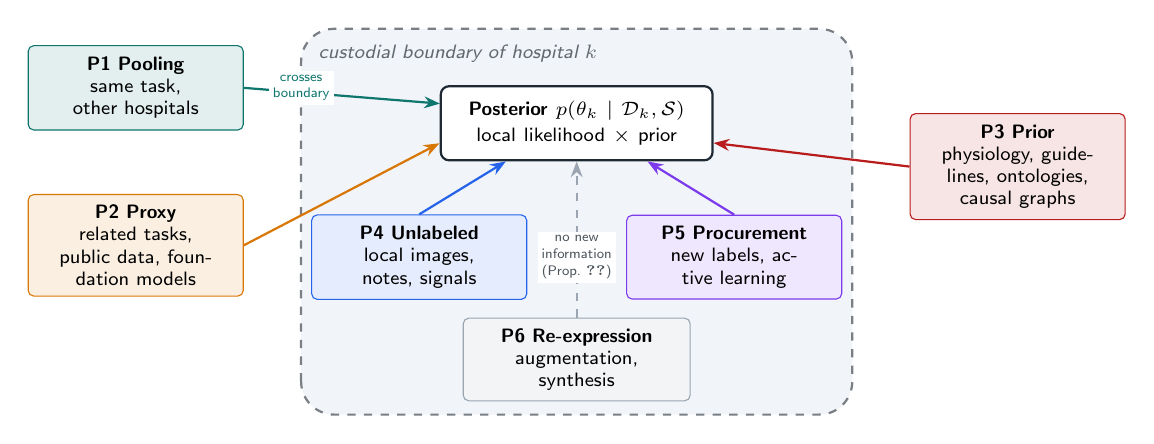
\begin{tikzpicture}[x=1bp,y=1bp,
  chan/.style={fill=#1!12,draw=#1,line width=0.4pt,rounded corners=2pt},
  ctxt/.style={align=center,font=\scriptsize\sffamily,inner sep=0pt,text width=2.4cm},
  flow/.style={draw=#1,line width=0.8pt,-{Stealth[length=2mm]}}]
\path[fill=slate100,draw=conc,line width=0.8pt,dashed,rounded corners=12pt] (-3.5cm,-3.15cm) rectangle (3.5cm,1.75cm);
\node[anchor=base west,font=\scriptsize\sffamily\itshape,text=edgec,inner sep=0pt] at (-93.06,38.98) {custodial boundary of hospital $k$};
\path[fill=white,draw=hdrc,line width=0.8pt,rounded corners=3pt] (-48.919,2.255) rectangle (48.919,28.935);
\node[align=center,font=\footnotesize\sffamily,inner sep=0pt,text width=3.1cm] at (0,15.595) {{\scriptsize\textbf{Posterior} $p(\theta_k \mid \mathcal{D}_k, \mathcal{S})$}\\ {\scriptsize local likelihood $\times$ prior}};
\path[chan=famE] (-95.404,-47.80) rectangle (-17.983,-17.399);
\path[chan=violetc] (17.983,-47.69) rectangle (95.404,-17.509);
\path[chan=grayc] (-40.84,-84.33) rectangle (40.84,-54.568);
\path[chan=famC] (-197.45,13.16) rectangle (-120.033,43.53);
\path[chan=famT] (-197.45,-46.62) rectangle (-120.033,-10.07);
\path[chan=famO] (120.033,-19.08) rectangle (197.45,19.08);
\node[ctxt] at (-56.694,-32.60) {\textbf{P4 Unlabeled}\\ local images, notes, signals};
\node[ctxt] at (56.694,-32.60) {\textbf{P5 Procurement}\\ new labels, active learning};
\node[ctxt,text width=2.6cm] at (0,-69.45) {\textbf{P6 Re-expression}\\ augmentation, synthesis};
\node[ctxt] at (-158.74,28.345) {\textbf{P1 Pooling}\\ same task, other hospitals};
\node[ctxt] at (-158.74,-28.345) {\textbf{P2 Proxy}\\ related tasks, public data, foundation models};
\node[ctxt] at (158.74,0) {\textbf{P3 Prior}\\ physiology, guidelines, ontologies, causal graphs};
\draw[flow=famC] (-119.833,28.347) -- (-49.24,22.67);
\node[fill=white,inner sep=1.5bp,align=center,font=\tiny\sffamily,text=famC] at (-99.214,28.347) {crosses\\ boundary};
\draw[flow=famT] (-119.833,-28.347) -- (-49.4,8.4);
\draw[flow=famO] (119.833,0) -- (49.3,8.5);
\draw[flow=famE] (-56.694,-17.199) -- (-25.5,1.85);
\draw[flow=violetc] (56.694,-17.309) -- (25.5,1.85);
\draw[flow=grayc,dashed] (0,-54.368) -- (0,1.85);
\node[fill=white,inner sep=1.5bp,align=center,font=\tiny\sffamily,text=gray600] at (0,-32.598) {no new\\ information\\ (Prop.~\ref{prop:nfl})};
\end{tikzpicture}}
\caption{The provenance axis. Each remedy draws information from one of six channels. Only pooling necessarily crosses the custodial boundary; only procurement adds fresh labeled observations from the target; re-expression adds no information about $\theta_k$ beyond what the local data and the generator already contain.}
\label{fig:provenance}
\end{figure*}

Two attributes of each channel matter for system design. The first is whether information crosses a custodial boundary, which determines the privacy cost: only P1 crosses one by necessity, and P2 does so when the proxy data belong to another custodian. The second is the source of bias: heterogeneity for P1, relevance for P2, misspecification for P3, the cluster or manifold assumption for P4, selection for P5 and generator bias for P6.

\subsection{Matching scarcity to provenance}\label{sec:matching}

The two axes together give a matrix (Figure~\ref{fig:matrix}) that answers a practical question: given the scarcity profile of a problem, which channels can in principle help? The entries are our judgment, informed by the mechanisms of Section~\ref{sec:provenance} and by the literature, graded from none to strong. They are claims about potential, not measurements, and Section~\ref{sec:evidence} sets them against where the coded corpus has actually worked (Figure~\ref{fig:gapmap}). Three patterns stand out. Ontic scarcity (O1 to O3) can only be addressed by pooling at a scale beyond the local site or by strong priors, since procurement is bounded by the world supply. Custodial scarcity (C1, C2) is addressed almost exclusively by pooling, which is why privacy-preserving pooling is the central technical problem for siloed healthcare. And re-expression is weak against every class, which follows from Proposition~\ref{prop:nfl} and matches the evidence.

The matrix is a set of claims about what can work in principle. The next three sections test it against what has actually been built and measured: Section~\ref{sec:method} describes how we assembled and coded the literature, Section~\ref{sec:solutions} reviews the methods channel by channel, and Section~\ref{sec:evidence} asks what the reported results, and the corpus as a whole, do and do not support.

\begin{figure}[t]
\centering
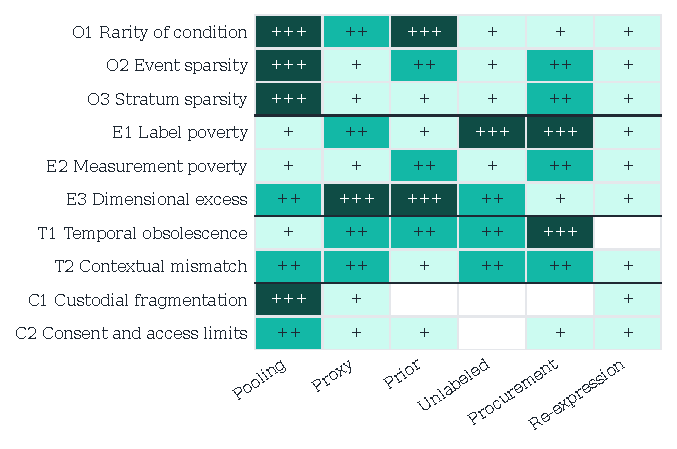
\includegraphics[width=0.66\linewidth]{figures/fig_matrix}
\caption{The Scarcity-Provenance matrix. Rows are the ten scarcity classes of Figure~\ref{fig:scarcity}; columns are the six provenance channels of Figure~\ref{fig:provenance}. Entries grade how strongly a channel can address a class (blank: not at all; $+$ weak; $++$ moderate; $+\,+\,+$ strong). Grades are the authors' judgment of potential; observed coverage in the coded corpus is shown in Figure~\ref{fig:gapmap}.}
\label{fig:matrix}
\end{figure}

%% ===================================================================
\section{Review Methodology}\label{sec:method}

The taxonomy gives us a vocabulary. To use it as a survey instrument, we need a body of literature coded in that vocabulary and an honest account of how it was assembled. This section provides both, following the guidelines of \citet{kitchenham2007guidelines} for literature reviews and of \citet{wohlin2014guidelines} for snowballing, and using PRISMA 2020 \cite{page2021prisma} as the reporting target.

\subsection{Research questions}

The review addresses five questions, each answered in a specific part of the paper.
\begin{enumerate}[label=\textbf{RQ\arabic*},leftmargin=*]
\item How can smallness be defined so that it is task-relative and measurable? (Section~\ref{sec:definition})
\item Which remedies exist for each scarcity class, and through which provenance channel do they import information? (Section~\ref{sec:solutions})
\item At what level are these remedies supported by evidence: theory, a single dataset, or data held by several institutions? (Section~\ref{sec:evidence})
\item Which combinations of scarcity class and channel that the taxonomy deems promising are under-studied? (Section~\ref{sec:evidence})
\item Which approach fits a sparse network of hospitals that cannot share records and has no trusted coordinator? (Section~\ref{sec:blueprint})
\end{enumerate}

\subsection{Corpus construction}

The corpus was assembled in two stages. The \emph{seed} set contained the foundational work for each provenance channel, the existing surveys listed in Section~\ref{sec:intro}, and the meta-research on clinical prediction models and medical imaging AI. The \emph{expansion} stage applied backward and forward snowballing \cite{wohlin2014guidelines} from the seed set, with the inclusion criteria below, until new candidates stopped adding channel and modality combinations not yet covered. Every record was checked against the publisher's page or a bibliographic index, and records whose details we could not confirm were dropped.

A work was included if it (I1) proposes, evaluates or reviews a way of learning from limited, fragmented or poorly labeled data, and either addresses health data directly or is the method that health applications build on; or (I2) documents, in health data, a failure or risk caused by scarcity, by distribution shift or by sharing. Works were excluded if they (X1) are textbooks, regulations or reporting guidelines; (X2) concern scaling with abundant data; or (X3) provide general learning theory not tied to a specific channel. Excluded works are still cited where they support an argument.

\begin{table}[t]
\caption{Coding scheme applied to every work in the corpus.}
\label{tab:coding}
\footnotesize
\begin{tabularx}{\linewidth}{@{}lp{2.5cm}X@{}}
\toprule
Attribute & Values & Rule\\
\midrule
Primary channel & P1 to P6, none & the channel through which most of the claimed information gain enters\\
Secondary channel & P1 to P6, empty & a second channel that is essential to the method, not incidental\\
Scarcity classes & O1 to C2, multi-label & the classes the work states it targets or documents, judged from its setting\\
Modality & imaging, EHR, tabular, text, omics, signals, multimodal, general & the data the work is evaluated on; general for methods not specific to health\\
Contribution type & method, theory, study, multi-site, resource, review, evidence & multi-site only if data come from two or more independent institutions\\
\bottomrule
\end{tabularx}
\end{table}

The bibliography has 335 entries; 45 are excluded background, which leaves a coded corpus of 290 works published between 1956 and 2025, 204 of them since 2019.

\subsection{Coding scheme}

Each work was coded on the five attributes of Table~\ref{tab:coding}. Channels and scarcity classes are those of Sections~\ref{sec:scarcity} and~\ref{sec:provenance}. A work has exactly one primary channel, the one through which most of its information gain is claimed, and at most one secondary channel; 48 of the 257 works that propose or study a remedy have one. Works that document a problem without proposing a remedy (33) are coded with the channel ``none''. Scarcity classes are multi-label and were assigned from the problem the work states it addresses and from its evaluation setting, not from what the method could do in principle. Contribution type records the primary contribution. A work is coded as a multi-site study only when its main contribution is training or validating on data held by two or more independent institutions; method papers that also report an external validation remain methods, and simulated partitions of a single dataset count as single-dataset evidence. The full coding is listed in Appendix~\ref{app:corpus} and released with the paper as a CSV file together with the scripts that produce every count and figure in Section~\ref{sec:evidence}.

\subsection{Threats to validity}

Four limitations qualify everything in the next two sections. First, \emph{the corpus is curated, not exhaustive}. It was built to cover every cell of the taxonomy and to support the argument of Section~\ref{sec:blueprint}, so pooling is over-represented by design (102 of 290 works), and counts describe the corpus, not the field. Absolute counts should not be compared across channels; the shape of coverage within a channel, and the cells that remain empty after a deliberate effort to fill them, are more informative. Second, \emph{coding was done by a single coder}, the first author, and inter-rater agreement has not been measured. Third, the primary channel is a judgment about where a method's gain comes from, and some works, foundation models trained with self-supervision for example, sit between two channels. Fourth, recent work is under-represented because of indexing and citation lag, so the decline after 2022 in Figure~\ref{fig:corpus} is not a trend.

\paragraph{Protocol for a systematic extension} To make the review systematic, we specify the search that would replace the curated stage. Databases: PubMed, Scopus, Web of Science, IEEE Xplore and the ACM Digital Library, with arXiv and medRxiv for preprints, from 2010 to the search date. Query, adapted to each database's syntax:
\begin{quote}
\footnotesize\ttfamily
("small data" OR "small sample*" OR "limited data" OR "data scarcity" OR "few-shot" OR "low-resource" OR "rare disease*" OR "label-efficient" OR "data-efficient" OR federated OR decentrali*ed OR "privacy-preserving") AND (health* OR clinical OR medic* OR hospital* OR patient*) AND ("machine learning" OR "deep learning" OR "transfer learning" OR "synthetic data" OR "data augmentation" OR "active learning" OR "semi-supervised" OR "self-supervised" OR "foundation model*" OR "hierarchical model*")
\end{quote}
Two reviewers screen titles and abstracts, then full texts, against criteria I1, I2 and X1 to X3, resolving disagreement by discussion and reporting Cohen's kappa; the same two reviewers code a random 20\% of included works independently to estimate coding reliability; and the flow is reported as a PRISMA 2020 diagram \cite{page2021prisma}.

\paragraph{Author note} This protocol has not yet been executed. All counts in Section~\ref{sec:evidence} and appendix~\ref{app:corpus} refer to the curated corpus described above. Before submission, the search should be run, the PRISMA flow added here, and the counts and figures regenerated from the resulting CSV with the scripts provided.

With the corpus defined, we turn to its content, channel by channel.

\section{Existing Solutions, Organized by Provenance}\label{sec:solutions}

 We now review solution families in the order of the provenance channels of Section~\ref{sec:provenance}. For each family we describe the mechanism, the scarcity classes of Figure~\ref{fig:scarcity} it addresses, the healthcare evidence, and the conditions under which it fails. Pooling receives the most space, because it is the only strong channel against custodial scarcity and therefore the foundation of Section~\ref{sec:blueprint}. Table~\ref{tab:families} gives a compact overview. By primary channel, the corpus holds 102 pooling, 60 proxy, 25 prior, 23 unlabeled, 15 procurement and 32 re-expression works, plus 33 that document a problem without proposing a remedy; Table~\ref{tab:corpus} in the appendix lists and codes every one of them.

\subsection{P1 Pooling: bringing the same task from other custodians}\label{sec:S6_1}

\paragraph{Centralized pooling and common data models} The simplest form of pooling is a shared repository. Public datasets such as MIMIC-III \cite{johnson2016mimic} have been central to the field precisely because they removed custodial scarcity for one population. Distributed networks built on common data models, such as OHDSI on the OMOP model \cite{hripcsak2015observational,overhage2012validation}, keep data local but harmonize their structure so that the same analysis can be run everywhere. Harmonization reduces C2 scarcity but does not by itself allow joint model fitting.

\paragraph{Distributed statistics} Long before federated learning, biostatistics developed ways to fit models across sites without moving records. Meta-analysis combines site-level estimates, and random-effects meta-analysis \cite{dersimonian1986meta} explicitly models between-site heterogeneity, a point we return to in Section~\ref{sec:blueprint}. Individual participant data meta-analysis is more powerful but needs record-level access \cite{riley2010meta}. Distributed regression exchanges sufficient statistics or gradients: GLORE fits logistic regression across sites by exchanging Newton-Raphson summaries \cite{wu2012grid}; DataSHIELD wraps such procedures in disclosure controls \cite{gaye2014datashield}; ODAL and related one-shot algorithms use surrogate likelihoods to obtain near-pooled estimates with one round of communication \cite{duan2020learning,jordan2019communication}; and the Personal Health Train infrastructure sends analyses to data stations rather than data to analyses \cite{beyan2020distributed}. \citet{jochems2016distributed} demonstrated a distributed model across hospitals in radiotherapy without any data leaving them. These methods are well understood, often exact, and auditable. Their limitation is model class: they work best for low-dimensional parametric models.

\paragraph{Federated learning} Federated averaging \cite{mcmahan2017communication} trains a shared model by alternating local gradient steps with server-side averaging. Healthcare adopted it quickly \cite{kaissis2020secure,nguyen2022federated,rieke2020future,xu2021federated}. Early work on institutional cyclical  training \cite{chang2018distributed} and on brain tumor segmentation showed that federated models could reach 99\% of the quality of a model trained on centrally pooled data \cite{sheller2020federated}. EXAM, trained across 20 institutions to predict oxygen needs of COVID-19 patients, improved average AUC by 16\% and generalisability by 38\% over single-site models \cite{dayan2021federated}. The largest study to date, across 71 sites and 6,314 glioblastoma patients, improved delineation of the surgically targetable tumor by 33\% over a model trained on public data \cite{pati2022federated}. FLamby provides seven cross-silo healthcare benchmarks with natural splits, which makes such claims testable \cite{ogierduterrail2022flamby}.

The central difficulty is heterogeneity. When site distributions differ, local updates drift apart and the averaged model can be worse than local ones \cite{hsieh2020non,zhao2018federated}. Remedies include proximal regularization (FedProx) \cite{li2020federated}, control variates (SCAFFOLD) \cite{karimireddy2020scaffold}, site-specific normalization (FedBN) \cite{li2021fedbn}, frequency-space augmentation for domain generalization (FedDG) \cite{liu2021feddg}, minimax objectives that protect the worst-off site \cite{mohri2019agnostic}, and ensemble distillation \cite{lin2020ensemble}. Medical versions of these ideas harmonize amplitude spectra and local drift across scanners \cite{jiang2022harmofl}, close the gap between federated and centralized segmentation on unseen sites \cite{xu2022closing}, adapt across acquisition sites in multi-site fMRI \cite{li2020multi}, and combine self-supervised pretraining with federated fine-tuning to tolerate heterogeneous, sparsely labeled sites \cite{yan2023label}. Federated transfer learning has also been applied to wearable sensor data \cite{chen2020fedhealth}, and federated tensor factorization and patient-similarity learning to EHR phenotyping \cite{kim2017federated,lee2018privacy}.

\paragraph{Clinical deployments} Beyond the landmark studies, the corpus contains a steady line of real multi-institution work. In structured EHR data, federated models have predicted hospitalizations from records held by separate custodians \cite{brisimi2018federated}, used patient clustering to cope with heterogeneous intensive care populations \cite{huang2019patient}, and predicted COVID-19 mortality across the hospitals of one health system \cite{vaid2021federated}. In imaging, federated training has been run across institutions for prostate segmentation \cite{sarma2021federated}, breast density classification \cite{roth2020federated}, COVID-19 diagnosis on CT \cite{bai2021advancing,dou2021federated}, and prediction of response to neoadjuvant chemotherapy in triple-negative breast cancer from whole-slide images \cite{ogierduterrail2023federated}; swarm learning has been applied to histopathology \cite{saldanha2022swarm}, and weakly supervised federated learning to gigapixel pathology \cite{lu2022federated}. The Personal Health Train trained a model on more than 20,000 lung cancer patients without moving their data \cite{deist2020distributed}, building on earlier distributed survival models in non-small cell lung cancer \cite{jochems2017developing}. At network scale, the OHDSI LEGEND study compared first-line antihypertensive classes across millions of patients in observational databases from several countries \cite{suchard2019comprehensive}, using a standardized framework for patient-level prediction \cite{reps2018design}, and web services made distributed logistic and Cox regression available to clinical researchers \cite{jiang2013webglore,lu2015webdisco}, with one-shot algorithms extending the approach to time-to-event outcomes \cite{duan2020learninglocal}. Most other pooling papers in the corpus, including several influential ones, evaluate on a single dataset partitioned to simulate sites \cite{guo2021multi,li2019privacy,sheller2019multi}. That distinction matters in Section~\ref{sec:evidence}.

\paragraph{Personalized federated learning} A more radical response is to stop looking for one model. Federated multi-task learning \cite{smith2017federated}, meta-learning based personalization \cite{fallah2020personalized}, Moreau-envelope regularization \cite{tdinh2020personalized}, Ditto \cite{li2021ditto}, shared representations with local heads (FedRep) \cite{collins2021exploiting}, mixtures of distributions \cite{marfoq2021federated}, attention-weighted collaboration among similar silos \cite{huang2021personalized} and clustered federated learning \cite{ghosh2020efficient} all learn a model per site while sharing statistical strength. \citet{tan2023personalized} survey the area. Theory on shared representations explains why this works when  sites share a low-dimensional structure \cite{baxter2000model,du2021few,maurer2016benefit,tripuraneni2020theory}.

\paragraph{Serverless and decentralized learning} Federated learning in its standard form assumes a central server that all sites trust to aggregate. Many hospital networks lack such an entity, or cannot agree on who should play it. Decentralized SGD replaces the server with neighbour averaging over a communication graph, and can match centralized rates when the graph mixes well \cite{koloskova2020unified,lian2017can,nedic2009distributed}. Gossip algorithms make this robust to asynchrony \cite{boyd2006randomized,xiao2004fast}. Personalized decentralized learning over a similarity graph was introduced by \citet{vanhaesebrouck2017decentralized} and extended with differential privacy by \citet{bellet2018personalized}. Cyffers and Bellet showed that decentralization itself amplifies privacy, because each party sees only what reaches it through the graph \cite{cyffers2022privacy}. In healthcare, Swarm Learning used a blockchain to coordinate peer-to-peer training without a central server across four clinical use cases \cite{warnatherresthal2021swarm}, and ProxyFL shares only differentially private proxy models among peers \cite{kalra2023decentralized}. Split learning partitions the network itself between parties \cite{gupta2018distributed,vepakomma2018split}, and vertical federated learning addresses the case where sites hold different features for the same patients \cite{yang2019federated}. Peer-to-peer training has been shown for brain segmentation \cite{roy2019braintorrent} and tumor segmentation in hospital networks \cite{tedeschini2022decentralized}, and split learning has been evaluated on clinical imaging tasks \cite{poirot2019split}. These healthcare demonstrations are few and mostly simulated, a gap that Section~\ref{sec:blueprint} addresses.

\paragraph{Privacy technologies} Sharing parameters or gradients is not private by default. Gradients can be inverted to reconstruct training images \cite{geiping2020inverting,zhu2019deep}, and trained models leak membership \cite{carlini2022membership,shokri2017membership}. Differential privacy (DP) \cite{dwork2006calibrating,dwork2014algorithmic} bounds what any output reveals about an individual and has been adapted to deep learning \cite{abadi2016deep,mironov2017renyi} and to federated training at the user or site level \cite{mcmahan2018learning,wei2020federated}. Secure aggregation reveals only the sum of updates \cite{bonawitz2017practical}; secure multi-party computation \cite{evans2018pragmatic} and homomorphic encryption \cite{gentry2009fully} allow computation on encrypted data, with multiparty homomorphic encryption demonstrated for federated analytics in precision medicine \cite{froelicher2021truly}. The costs are well known. DP degrades accuracy, more so for small datasets, high-dimensional models and under-represented groups \cite{bagdasaryan2019differential,jayaraman2019evaluating,tramer2021differentially}. Cryptographic methods protect the computation but not what the final model reveals. Robust aggregation protects against malicious participants \cite{blanchard2017machine}. In healthcare, end-to-end privacy-preserving training combining secure aggregation and DP was demonstrated on pediatric chest radiographs \cite{kaissis2021end}, DP has been studied for medical imaging \cite{ziller2021medical} and for federated pathology \cite{adnan2022federated} and EHR models \cite{choudhury2019differential}, and cryptographic systems support distributed cohort exploration \cite{raisaro2019medco} and genome-wide association studies \cite{cho2018secure}. The threat is concrete. Gradient inversion has been demonstrated on medical federated training, with risk governed by batch size and the number of local steps \cite{hatamizadeh2023do}; deep networks can re-identify patients from chest radiographs \cite{packhauser2022deep}; face-recognition software can identify research participants from MRI \cite{schwarz2019identification}; and re-identification attacks on health data have a long record \cite{elemam2011systematic}.

\subsection{P2 Proxy: borrowing from related tasks}\label{sec:S6_2}

\paragraph{Transfer learning} Pretraining on a large source and fine-tuning on a small target is the most widely used remedy \cite{pan2010survey}. Its value in medical imaging is more nuanced than often  assumed. Raghu et al. found that ImageNet pretraining gave little performance benefit on large medical imaging tasks and that much smaller architectures performed comparably, with the benefit concentrated in faster convergence and in the smallest data regimes \cite{raghu2019transfusion}. Domain adaptation theory gives the reason: the target risk is bounded by the source risk plus a divergence between domains and the error of the best joint hypothesis \cite{bendavid2010theory}. When the proxy is far from the target, these terms dominate. Earlier empirical studies on medical images found that fine-tuning a pretrained network performed at least as well as training from scratch and was more robust to reductions in training data \cite{shin2016deep,tajbakhsh2016convolutional}, and the specialist-level results on skin and retinal images were themselves fine-tuned ImageNet models trained on large labeled sets \cite{esteva2017dermatologist,gulshan2016development}. Medical sources make the proxy closer: 3D pretraining on aggregated segmentation datasets \cite{chen2019med3d}, self-supervised Models Genesis \cite{zhou2021models} and the RadImageNet database \cite{mei2022radimagenet} all aim at this, and domain adaptation methods target the remaining shift directly \cite{guan2022domain,kamnitsas2017unsupervised}.

\paragraph{Self-supervised and foundation models} Self-supervised pretraining by contrastive learning \cite{chen2020simple} or masked reconstruction \cite{he2022masked} removes the need for source labels and allows pretraining on in-domain unlabeled data. Azizi et al. showed that self-supervised pretraining on unlabeled medical images improved top-1 accuracy by 6.7\% on dermatology classification and mean AUC by 1.1\% on chest X-ray classification over supervised ImageNet pretraining \cite{azizi2021big}. RETFound, pretrained on 1.6 million unlabeled retinal images, adapted to ocular and systemic disease detection with fewer labels than comparison models \cite{zhou2023foundation}. Vision-language pretraining \cite{radford2021learning,wang2022medclip}, large language models that encode clinical knowledge \cite{singhal2023large} or extract clinical information from few examples \cite{agrawal2022large}, and EHR foundation models \cite{rasmy2021med,steinberg2021language} extend the idea across modalities; \citet{moor2023foundation} argue for generalist medical models, and \citet{bommasani2021opportunities} discuss their risks. Medical image-text pretraining \cite{huang2021gloria,zhang2022contrastive} and contrastive pretraining on chest radiographs \cite{sowrirajan2021moco} improve label efficiency, and a model trained only on radiographs paired with their reports detected several pathologies at expert level without explicit labels \cite{tiu2022expert}. Computational pathology has seen the fastest growth, with general-purpose slide and tile encoders \cite{chen2024general,xu2024whole}, vision-language models \cite{lu2024visual}, and a foundation model that reported clinical-grade detection of rare cancers \cite{vorontsov2024foundation}; segmentation \cite{ma2024segment} and cancer imaging biomarkers in limited-data settings \cite{pai2024foundation} follow the same pattern. For EHR, sequence models pretrained on large patient histories \cite{choi2016doctor,li2020behrt} and a health-system scale language model trained on clinical notes \cite{jiang2023health} transfer to many prediction tasks, although a review of EHR foundation models found evaluations narrow and rarely tied to clinical value \cite{wornow2023shaky}. Clinical and biomedical language models \cite{alsentzer2019publicly,lee2020biobert} and general large language models \cite{nori2023capabilities} bring textual knowledge, and transcriptomic foundation models pretrained on tens of millions of single cells transfer to settings with few samples \cite{cui2024scgpt,theodoris2023transfer}. Parameter-efficient fine-tuning \cite{hu2022lora} reduces the number of parameters to adapt, which lowers $n^{\star}$ directly.

\paragraph{Tabular data} Much of healthcare is tabular, where deep learning has a weaker record. Tree ensembles still outperform deep networks on typical medium-sized tabular benchmarks \cite{grinsztajn2022do}. Two recent lines are directly about small data. TabPFN is a transformer trained only on synthetic datasets drawn from a prior over structural causal models, which performs Bayesian inference in a single forward pass \cite{hollmann2023tabpfn}; its second version outperformed an ensemble of strong baselines tuned for four hours, in 2.8 seconds, on datasets of up to 10,000 samples \cite{hollmann2025accurate}. In the language of our taxonomy, it converts a prior (P3) into a proxy (P2)
 by sampling. TabLLM serializes rows into text and uses a large language model’s knowledge for few-shot classification \cite{hegselmann2023tabllm}, drawing on prior knowledge absorbed during pretraining. Both point to a general principle: in the small regime, the quality of the prior matters more than the flexibility of the model.

\paragraph{Few-shot and meta-learning} Meta-learning learns an inductive bias from a distribution of related tasks, so that a new task can be learned from few examples \cite{baxter2000model,finn2017model,hospedales2022meta,snell2017prototypical,wang2020generalizing}. Its assumptions are demanding: many related training tasks drawn from the same distribution as the target task. In healthcare that distribution is often what is missing. Medical applications exist for clinical risk prediction from limited EHR \cite{zhang2019metapred}, rare skin conditions \cite{mahajan2020meta,prabhu2019few} and volumetric segmentation from few annotated scans \cite{roy2020squeeze}, and facial-phenotype models for rare genetic syndromes \cite{gurovich2019identifying,hsieh2022gestaltmatcher} show how a proxy trained on many syndromes can support conditions with only a handful of known patients.

\subsection{P3 Prior: knowledge that is not data}\label{sec:S6_3}

\paragraph{Bayesian and hierarchical modeling} Bayesian inference makes the prior explicit \cite{gelman2013bayesian}. Hierarchical models are the canonical way to share strength across groups, and their frequentist counterpart, shrinkage, is provably better than separate estimation in three or more dimensions \cite{efron1973steins,stein1956inadmissibility}. Penalized regression \cite{hastie2009elements,tibshirani1996regression} is the prior in disguise, and its use is recommended for small clinical prediction datasets, although it does not replace adequate sample size \cite{riley2020calculating,smeden2019sample}. The clinical evidence is more cautious than the theory. Shrinkage improved small-sample prognostic models in early comparisons \cite{steyerberg2000prognostic}, but later studies showed that it does not guarantee better performance and is least reliable precisely when samples are smallest, because the amount of shrinkage is itself estimated with large uncertainty \cite{riley2021penalization,vancalster2020regression}. This is the same problem that the blueprint of Section~\ref{sec:blueprint} faces when it estimates the heterogeneity $\tau^2$, and Proposition~\ref{prop:borrowing} quantifies it.

\paragraph{Mechanistic and physics-informed models} When the system has known dynamics, as in pharmacokinetics, cardiovascular hemodynamics or tumor growth, embedding them as constraints or residuals dramatically reduces the data needed \cite{karniadakis2021physics,raissi2019physics}. \citet{rueden2023informed} classify how knowledge can enter learning: through the training data, the hypothesis set, the learning algorithm or the final hypothesis. Medical examples include physics-informed networks for cardiac activation mapping \cite{sahlicostabal2020physics} and arterial blood pressure \cite{kissas2020machine}, biologically informed networks for sparse experimental data \cite{lagergren2020biologically}, and neural ordinary differential equations for pharmacokinetics \cite{lu2021neural}. Human concept learning from one example, formalized as probabilistic program induction \cite{lake2015human}, is the limiting case of what a strong prior can do.

\paragraph{Ontologies and knowledge graphs} Medical codes are organized in hierarchies. GRAM uses these ontologies to give rare codes representations close to their ancestors, improving prediction for codes that appear only a few times \cite{choi2017gram}. This directly targets the long tail created by E3 and O1. KAME and GAMENet extend the idea with knowledge-graph attention and drug-interaction graphs \cite{ma2018kame,shang2019gamenet}, health knowledge graphs can be learned from records \cite{rotmensch2017learning}, and the Human Phenotype Ontology \cite{kohler2021human} supplies the structured vocabulary that rare-disease models rely on.

\paragraph{Causal knowledge} Causal structure tells a model which relations should be stable across sites and time. Invariance-based learning \cite{arjovsky2019invariant}, causal representation learning \cite{pearl2009causality,scholkopf2021causal}
  and causal analysis of imaging datasets \cite{castro2020causality} target T1 and T2 scarcity by excluding features whose relation to the outcome is site-specific. Graphical models of the shift itself can identify which relations will transport \cite{subbaswamy2019preventing}. The empirical record is sobering, however: under careful model selection, domain generalization methods did not consistently beat plain empirical risk minimization, either on general benchmarks \cite{gulrajani2021search} or in clinical settings \cite{zhang2021empirical}.

\subsection{P4 Unlabeled: information in the inputs}\label{sec:S6_4}

 Semi-supervised methods such as consistency regularization with pseudo-labels \cite{sohn2020fixmatch} use unlabeled inputs to shape the decision boundary. \citet{cheplygina2019not} review semi-supervised, multiple-instance and transfer learning in medical imaging, and \citet{tajbakhsh2020embracing} review solutions for imperfect segmentation datasets. Weak supervision builds noisy labels from heuristics, knowledge bases and existing records and combines them with a generative label model \cite{ratner2017snorkel}. As Proposition~\ref{prop:nfl} and the causal analysis of \citet{scholkopf2012causal} imply, these methods help when the input distribution carries information about the label mechanism. They are effective against E1 and much less so against O-type scarcity.

In medical image segmentation, semi-supervised learning has been developed through self-training \cite{bai2017semi}, uncertainty-aware and transformation-consistent self-ensembling \cite{li2021transformation,yu2019uncertainty}, and contrastive pretraining on the unlabeled part of the same dataset \cite{chaitanya2020contrastive,taleb20203d}, with few-shot segmentation trained from superpixels without annotation \cite{ouyang2020self}; \citet{krishnan2022self} review self-supervision in medicine. In computational pathology, attention-based multiple-instance learning \cite{ilse2018attention} made slide-level labels sufficient: a system trained on tens of thousands of slides with only diagnostic labels reached clinical-grade performance \cite{campanella2019clinical}, and CLAM made the approach data-efficient \cite{lu2021data}. Large chest radiograph datasets were labeled by mining radiology reports \cite{irvin2019chexpert,wang2017chestx}, which trades label poverty (E1) for measurable label noise (E2). In EHR data, anchor-based phenotyping \cite{halpern2016electronic}, learning from noisy labels \cite{agarwal2016learning} and weak supervision of clinical text \cite{fries2019weakly,wang2019clinical} play the same role.

\subsection{P5 Procurement: acquiring the right new data}\label{sec:S6_5}

 Procurement is the most neglected channel in machine learning papers and the most important one in clinical research. Sample size calculations \cite{riley2020calculating} turn smallness into a design problem before data collection starts. Active learning chooses which examples to label next to maximize information \cite{settles2009active}, and has been widely studied in medical imaging \cite{budd2021survey}. Representative methods select annotation regions by uncertainty and representativeness \cite{yang2017suggestive}, use learned feature distances \cite{smailagic2018medal}, or exploit Bayesian uncertainty \cite{gal2017deep,nath2021diminishing}. Learning curves fitted on pilot data can predict how many labeled examples a target accuracy needs \cite{cho2015much,figueroa2012predicting}, and \citet{balki2019sample} review sample-size methods for machine learning in imaging; for continuous outcomes the clinical criteria have their own form \cite{riley2019minimum}. Procurement is the smallest channel in our corpus (15 works), which is at odds with its importance. Data valuation methods such as Data Shapley \cite{ghorbani2019data} estimate which records or sources contribute most, which could guide both acquisition and the fair crediting of contributors in a consortium.

\subsection{P6 Re-expression: augmentation and synthetic data}\label{sec:S6_6}

 Data augmentation encodes invariances and is standard practice \cite{shorten2019survey,zhang2018mixup}. Oversampling methods such as SMOTE \cite{chawla2002smote} interpolate minority  examples. Deep generative models, from GANs \cite{goodfellow2014generative} to diffusion models \cite{ho2020denoising,kazerouni2023diffusion}, can produce realistic medical images, and tabular and EHR generators include medGAN \cite{choi2017generating} and CTGAN \cite{xu2019modeling}. In a widely cited study, GAN-based augmentation improved liver lesion classification from 78.6\% to 85.7\% sensitivity and from 88.4\% to 92.4\% specificity on a dataset of 182 lesions \cite{fridadar2018gan}. Similar results have been reported for brain MRI synthesis used for both augmentation and anonymization \cite{shin2018medical}, for segmentation \cite{bowles2018gan}, for 3D generation with diffusion models \cite{khader2023denoising}, and for learned spatial and appearance transformations that make one-shot segmentation possible \cite{chaitanya2021semi,zhao2019data}; \citet{yi2019generative} and \citet{chlap2021review} review the area. A large study found that diffusion-based augmentation improved fairness and robustness of medical classifiers under distribution shift \cite{ktena2024generative}; in our terms, the information came from the generator’s training data, not from the act of sampling. For structured records, EHR generators \cite{baowaly2019synthesizing,zhang2020ensuring}, anonymization-oriented synthesis \cite{beaulieujones2019privacy,yoon2020anonymization}, diffusion and language-model tabular generators \cite{borisov2023language,kotelnikov2023tabddpm}, and the rule-based Synthea simulator \cite{walonoski2018synthea} have been proposed and evaluated \cite{goncalves2020generation}. Rebalancing deserves a warning: in clinical risk prediction, class imbalance corrections produced badly calibrated risks without improving discrimination \cite{goorbergh2022harm}, despite their popularity \cite{fernandez2018smote}.

Synthetic data are also promoted as a privacy technology \cite{chen2021synthetic,jordon2022synthetic}. Here the evidence is sobering. Stadler et al. found that synthetic data either fail to protect against linkage and attribute inference or lose much of their utility, and do not provide a better privacy-utility trade-off than traditional anonymization \cite{stadler2022synthetic}. Formally private generators such as PATE-GAN \cite{jordon2019pate}, built on the PATE framework \cite{papernot2017semi}, provide guarantees at the cost of fidelity. And recursive training on generated data causes models to lose the tails of the distribution \cite{shumailov2024ai}, which in healthcare are exactly the rare cases and minority groups that motivated the effort. Proposition~\ref{prop:nfl} summarizes the position: synthetic data are a useful vehicle for information that already exists (in a pretrained generator, or in another site’s data under a privacy guarantee), but not a source of it.

Taken together, the six channels cover a wide range of techniques, but the evidence behind them is uneven. Some channels have been tested at multi-site scale, others mainly on internal splits of a single dataset. The next section reads the reported results through the taxonomy to separate the two.


%%CHUNK4%%

\bibliographystyle{ACM-Reference-Format-recovered}
\bibliography{references}

\end{document}
